\subsection{Ocena gostote verjetnosti z jedrom}
Opišimo še nekoliko drugačen pristop za predstavitev podatkov. Najprej pa moramo povedati, kaj sploh mislimo z besedo "jedro".
\begin{definicija}
    \textbf{Jedro} je nenegativna realna integrabilna funkcija $K$ z lastnostima:
    \begin{itemize}
        \item $\int_{-\infty}^\infty K(x) \  dx = 1 \quad$ in
		\item $K(-x) = K(x), \quad \forall x \in \mathbb{R} \quad$ (simetrija).
    \end{itemize}
\end{definicija}

\begin{figure}[!h]
    \centering
    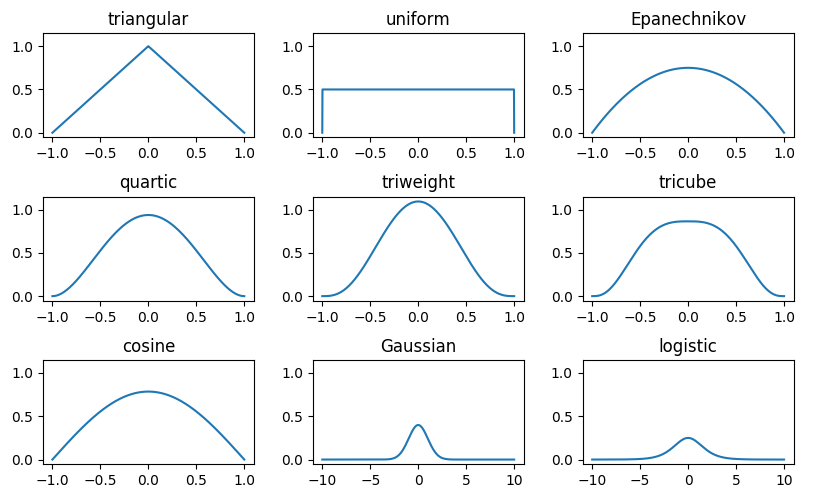
\includegraphics[width=\textwidth]{jedra.png}
    \caption{Nekaj primerov jeder.}
    \label{jedra}
\end{figure}

Ideja ocenjevanja gostote verjetnosti z jedri (angl. \textit{kernel density estimation}) je, da na vsako točko v vzorcu obesimo jedro, ki ga vnaprej določimo, nato pa ta jedra seštejemo in rezultat normiramo. Ker so jedra nenegativna, bo torej pridobljena funkcija ustrezala definiciji gostote verjetnosti.
\begin{definicija}
    \textbf{Ocena gostote verjetnosti z jedrom} je neparametričen način ocenjevanja gostote verjetnosti. Naj bo $K$ jedro in $X = \{x_1,\ldots,x_n\}$ množica podatkov.  Ocena gostote verjetnosti z jedrom $K$ množice $X$ je funkcija, definirana kot:
    \begin{equation}
        f_h(x) = \frac{1}{n\cdot h} \  \sum_{i=1}^n K\Big(\frac{x - x_i}{h}\Big),
    \end{equation}
    kjer je $h$ parameter glajenja, imenovan "bandwidth". % bandwidth == pasovna širina?? mislim da ne
\end{definicija}

Parameter $h$ močno vpliva na končno oceno. Če je $h$ premajhen, lahko dobimo močno oscilirajočo funkcijo, ob preveliki izbiri $h$ pa lahko izgubimo pomembne podatke o porazdelitvi. Če potegnemo vzporednico s podpoglavjem o histogramih, lahko rečemo, da $h$ igra podobno vlogo kot izbira optimalnega števila stolpcev pri histogramih. V optimizacijo paramtra $h$ se ne bomo poglabljali, ponavadi pa ga izračunamo kot:
\begin{equation}
    h = \sigma(X) \cdot \Big(\frac{4}{3|X|}\Big)^{1/5},
\end{equation}
kjer je $\sigma(X)$ standardni odklon množice podatkov $X$.

Pri ocenjevanju gostote verjetnosti z Gaussovim jedrom uporabljamo Gaussovo jedro (slika \ref{jedra}). To je normalna porazdelitev s srednjo vrednostjo 0 in varianco 1, torej:
\begin{equation}
	K(x) = \frac{1}{\sqrt{2\pi}}e^{-\frac{1}{2}x^2}.
\end{equation}
Ocenjevanje gostote verjetnosti z Gaussovim jedrom smo izpostavili, ker je zelo pogost. Poleg tega je zelo dobra ocena pri porazdelitvah s trebuhi (npr. normalna porazdelitev, Rayleigh porazdelitev, ...). Je pa ta metoda zelo slaba pri porazdelitev s končnimi nosilci (npr. uniformna podrazdelitev), saj zaradi neomejenosti definicijskega območja Gaussovega jedra funkcija, ki jo dobimo z oceno, preseže ta nosilec.

\begin{figure}[!h]
    \centering
    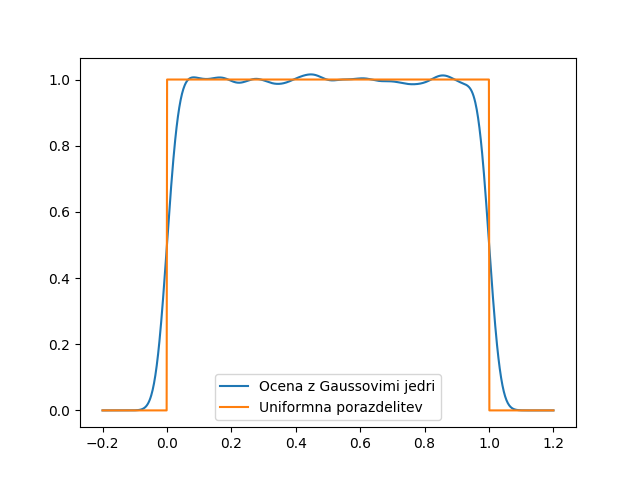
\includegraphics[width=0.45\textwidth]{gaussVSuniform.png}
    \caption{Vidi se, da ocena z Gaussovimi jedri preseže nosilec uniformne porazdelitve.}
\end{figure}
\pagebreak
Predstavili smo dva načina predstavitve podatkov. Obe načina predstavitve imata svoje prednosti in slabosti. Predstavitev s histogrami je zelo kompaktna, poleg tega pa histogram nikoli ne bo segal ven iz nosilca porazdelitve, saj je omejen s podatkovno množico. Pri ocenjevanju gostote verjetnosti z jedri se pa lahko zelo dobro približamo porazdelitvi, ki jo podatki predstavljajo, s čimer ne bomo izgubili nobene pomembne lastnosti podatkovne množice. Tvegamo pa, da lahko pademo ven iz nosilca.

Za naključen set podatkov, o katerem ne vemo nič, je težko reči, kateri način predstavitve je boljši. Vemo pa, da je za porazdelitve, ki imajo neskončne nosilce $(-\infty, \infty)$ in so gladke, veliko boljša predstavitev z oceno z Gaussovimi jedri. Pri porazdelitvah z omejenimi nosilci pa ta možnost odpade, tako da smo primorani operirati s histogrami.

Za konec tega poglavja pa predstavimo način, kako lahko optimalno število stolpcev iščemo z uporabo divergence. Kot primer vzemimo kar Kullback-Leibler divergenco $D_{KL}$.